\part{Project Description}

\chapter{High level}
The project consists in creating a mobile application aimed at connecting people to make daily trips. This app is close to other apps carpool like BlaBlaCar for example, but it favors mainly course and regular trips.
\\The application is part of the eco-responsibility domain. Indeed, we often notice that vehicles traveling in cities contain only one person. Carpooling offers significant advantages: to meet new people, to divide the journey price by the number of passengers, and of course to reduce the number of cars on the island, so the pollution but also the amount of traffic jams. The car traffic will be smoother and you will spend less time on the road. Indeed, the traffic on the island of Malta is difficult, the roads are narrow and old. The infrastructure of the Maltese roads is not suitable for such a high number of cars, especially in the summer when the island welcomes many tourists, 2.2 million expected for 2018.
\\The app favors drivers. They must not wait or make a detour, theoretically of course, free to them to be accommodating. It is the passenger who must be at a given time and a given position. Knowing that the driver and the passenger will have a different path, the application will find the closest driver and calculate the distance to reach the meeting point.{\bf CCcomment: if would be great if you could add some figures and examples of maps}
\\The application is intended to connect drivers and passengers only, it will not deal with the management of payments, if any, or the management of places. The app will track driver's journeys and suggest the one that's best for users seeking a ride. The application must be simple and intuitive.

\chapter{Technical description}
This application will be available on iOS and Android platform. The client-server environment refers to a mode of communication across a network between several programs: one, qualified as a client, sends requests; the other , qualified as server wait for and respond to customer requests.

\begin{figure}[h]
\centering
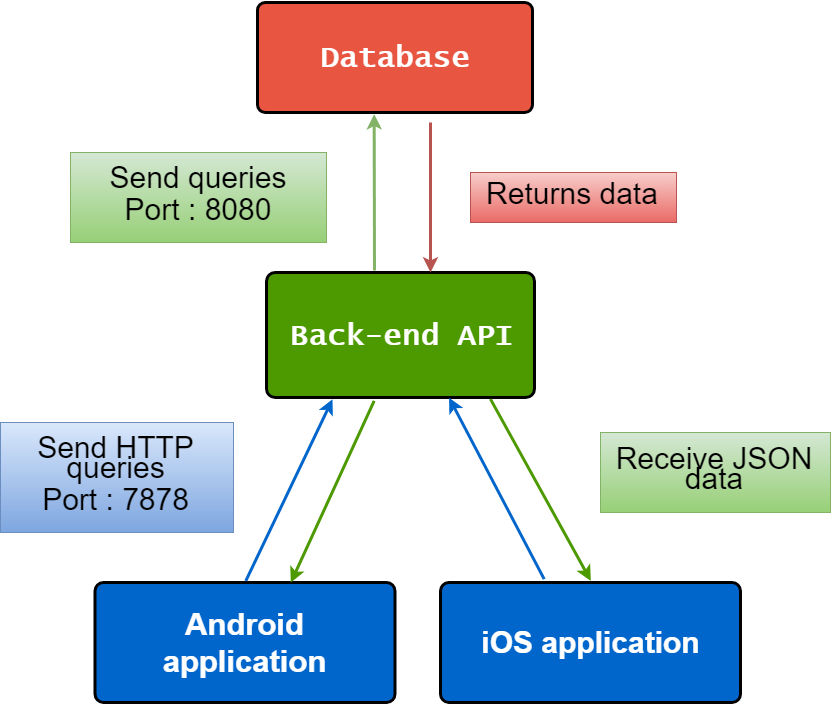
\includegraphics[scale=0.40]{diagrams/connecting_parts.png}
\caption{Diagram showing the architecture of the project}
\end{figure}

This chapter is divided in 5 majors subparts :
\begin{itemize}
    \item Back-end API
    \item Database settings
    \item How to use
    \item Search algorithm
    \item Application design
\end{itemize}

\section{Back-end API}
The back-end server is an API using the NodeJS (JavaScript) technology. It is related to a database using MySQL to store the data of the application. The clients send HTTP request to the server, which answer back some datas. This is how the clients and the server communicate. The chapter 3 list all of the functions available on the back-end API.

\section{Database settings}
The database is using MySQL and PHPMyAdmin to interact with. The database is composed of 8 tables :
\begin{itemize}
    \item \textbf{User} : This table store all the users data.
    \begin{itemize}
    	\item id : The ID of the user
    	\item username : The user's username
    	\item password : User's password
    	\item name : User's first name
    	\item surname : User's last name
    	\item email	: User's email
    	\item mobileNumber : User's mobile number
    	\item isVerified : Is the user verified ?
    \end{itemize}
    \item \textbf{Route} : This table store all the routes created by the users.
    \begin{itemize}
    	\item id : The ID of the route
    	\item startingPoint : The geographical point at the beginning of the route
    	\item endPoint : The geographical point at the end of the route
    	\item driver : The user id that created this route
    	\item originAdress : The adress of the origin of the route
    	\item destinationAdress	: The adress of the destination of the route
    	\item distance : The distance between the origin and the destination of the route (in meters)
    	\item duration : The duration of the route (in seconds)
    \end{itemize}
    \item \textbf{RouteDate} : This table associate a route with a date. This date represents the starting time of the driver.
    \begin{itemize}
    	\item id : The ID of the route meta line
    	\item route : The route ID linked to this meta
    	\item route\textunderscore date : First date of the repeat. It's assumed to be every week starting from this day
    	\item weekly\textunderscore repeat : Is this route must be repeated every week ?
    \end{itemize}
    \item \textbf{RoutePoints} : This table is the heaviest of the database. It stores every key points of every routes. Routes are divided in RoutePoints, which fits the path of the driver.
    \begin{itemize}
    	\item id : The ID of the route point
    	\item route : The route ID linked to this point
    	\item point\textunderscore rank : It's the order of this point in the point list of the route
    	\item point : The geographical coordinates of this point
    	\item square\textunderscore id\textunderscore lng : The longitude id of the square of the routePoint
    	\item square\textunderscore id\textunderscore lat : The latitude id of the square of the routePoint
    	\item seconds\textunderscore from\textunderscore start : An estimation of the number of seconds passed since the start of the route
    \end{itemize}
    \item \textbf{Ride} : A ride is an instance of a route.
    \begin{itemize}
    	\item id : The ID of the ride
    	\item route : The route attached to this ride
    \end{itemize}
    \item \textbf{Rating} : This table store the rates of the users.
    \begin{itemize}
    	\item id : The comment ID
    	\item author : The user ID of the author of the comment
    	\item target : The user ID of the target of the comment
    	\item ride : The ride ID linked to this comment
    	\item stars : How many stars did the author reward the target ?
    	\item comment : The text content of the comment
    	\item postDate : The date of the rate
    \end{itemize}
    \item \textbf{Passenger} : This table associate a passenger to a driver's route.
    \begin{itemize}
    	\item id : The ID of the row
    	\item ride : The ride ID linked to the passenger
    	\item passenger : The passenger ID linked to the route
    \end{itemize}
    \item \textbf{FavoriteRoute} : This table is used to add some favorites routes.
	\begin{itemize}
    	\item id : The ID of the row
    	\item routeId : The route attached to this save
    	\item userId : The user attached to this save
    \end{itemize}
\end{itemize}

\section{How to use}

\subsection{Set-up the backend API}
First, to set up the backend API, you need to be be connected to the remote server, by ssh. To connect by ssh, you have to write in a command prompt :

\begin{lstlisting}[style=DOS]
user@desktop:~$ ssh username@ip_server
\end{lstlisting}

Then, using git, clone the github's repository :
\begin{lstlisting}[style=DOS]
user@desktop:~$ git clone https://github.com/ccol002/getalift.git
\end{lstlisting}

Finally, you need to start the server using npm :
\begin{lstlisting}[style=DOS]
user@desktop:~$ cd getalift/getalift_backend
user@desktop:~/getalift/getalift_backend$ npm start
\end{lstlisting}

Once you will see the following displayed in the console, it will mean that the server is ready.

\begin{lstlisting}[style=DOS]
> getalift-backend@0.0.0 start /home/user/getalift/getalift_backend
> node index.js

[S] Server is listening on port 7878.
\end{lstlisting}

\subsection{Set-up the database}
To set-up the database, you need to connect to phpmyadmin through the following URL :

\begin{lstlisting}[style=DOS]
http://ip_server/phpmyadmin/index.php
\end{lstlisting}

The username is "root", and the password is also "root". Then, to create the database, import the script "database.sql" located in the getalift\textunderscore backend folder.

\subsection{Interact with the backend API}

To interact with the API, use Postman. Postman is a complete API development environment, for API developers, used by more than 5 million developers and 100000 companies worldwide. With Postman, you can send HTTP request to the api, and see the response.

If the request is POST, or PUT, you need to set some keys in the body part of the request. Theses key depends of the route of the request, you can find all theses parameters details in the getalift\textunderscore backend/index.js file.

Note : The API is securised with json web token. For all the requestw made to the API, you need to set a key "x-access-token" in the header part of the request, and the value of this key have to be a valid token. A valid token is delivered in the response of successful authentication request to the API. There is only 2 routes that can be reached without token, the authentication and the register route.

\section{Search algorithm}

To find the best driver's route that match with the passenger's route, a search algorithm has been created. The biggest challenge was to try to find the best route, with an answer time lower than 1 second. To launch this algorithm, we need 5 parameters :

\begin{itemize}
    	\item startLat : The latitude of the starting point of the passenger
    	\item startLng : The longitude of the starting point of the passenger
    	\item endLat : The latitude of the ending point of the passenger
    	\item endLng : The longitude of the ending point of the passenger
    	\item startDate : The date where the passenger is able to start travelling
\end{itemize}


\subsection{Part 1 : Square ID selection}
Knowing that the numbers of routes in the database can be huge, this first step goal is to refine the numbers of routes that I will analyze in step 2.

We divided the world map into squares of 500 meters square approximately. All theses squares have unique square ID. To create a unique identifier to every square, the square ID will be composed of 2 elements : the latitude ID and the longitude ID.  Each time a driver add a route to the database, for every routePoints of the route, the square ID is calculated and stored into the database.

Then, we know the starting point and the ending point of the passenger. So we calculate the square ID of theses 2 points. And we look in the database, for all the routes that matches theses two conditions :
\begin{itemize}
	\item The route have a routePoint with the same squareID than the starting point of the passenger
	\item The route have a routePoint with the same squareID than the ending point of the passenger
\end{itemize}


\subsection{Part 2 : Vector direction angle}

All the routes that passed the first step and that their startingDate is older than the startDate of the passenger are subjected to this second step. This step is use to hold only the routes that goes in the same direction than the passenger. Why ? Because, for example, if a driver move from A to B, and the passenger move from B to A, the driver's route will pass the first step, but this route is not interesting for the passenger because it is the inverse route.

For each routes, I create two vectors. One from the starting point to the ending point of the driver. 
And the other one from the starting point to the ending point of the passenger.
Then, I am calculating the angle between the two vectors, and I hold only routes where the angle is less than 90 degrees.

\subsection{Part 3 : K-d tree algorithm}

All the routes that passed the second step are subjected to this third step. This is the last step. This step goal is to find the x routes which have routePoints close to the passenger key points.

A k-d tree is a space-partitioning data structure for organizing points in a k-dimensional space.
K-d trees are a useful data structure for several applications, such as searches involving a multidimensional search key. It is used to find the closest neighbors
of a point. I am using it to find, for each routes, the closest routePoint of the driver depending on the passenger starting point. Idem for the passenger ending point.

Then, the routes array is sorted by totalDisance (increasing), and the 3 first elements of this array are returned using JSON. Here is the JSON format returned :

\begin{lstlisting}[style=DOS]
{
	[Array of routes]
}
\end{lstlisting}

A route is defined by :
\begin{lstlisting}[style=DOS]
{
	"id" : the ID of the route,
	"closestPointStart" : the routePoint of the route that is the closest to the
		passenger starting point,
	"closestPointEnd" : the routePoint of the route that is the closest to the 
		passenger ending point,
	"distancePointStart" : the distance in meters between the passenger starting 
		point and the closestPointStart,
	"distancePointEnd" : the distance in meters between the passenger ending point
		and the closestPointEnd,
	"totalDistance" : the sum of the two above distances (in meters),
	"user_id" : the user ID of the route's driver,
	"user_name" : the username of the route's driver,
	"route_date" : the starting time of the driver's route,
	"routePoints" : an array of all the routePoints of the route
}
\end{lstlisting}

A routePoint is defined by :
\begin{lstlisting}[style=DOS]
{
	"id" : the ID of the routePoint,
	"point" : {
		"x" : the latitude of the point,
		"y" : the longitude of the point
	},
	"route" : the route ID,
	"seconds_from_start" : an estimation of the number of seconds
		passed since the start of the route
}
\end{lstlisting}


\section{Application design}

The following page is the application design realised by Loan AUBERGEON. Here is a description the design :

\begin{itemize}
	\item {\bf Page 1 : Login}. This is the first page of the application. It is used to either log the user, or he also can create an account by clicking on the button "Create an account"
	\item {\bf Page 2 : Sign in}. This page is use to register the user in the database. 
	\item {\bf Page 3 : Home}. This is the home page of the application. There is a map from Google Map in the background, focused on the user's localisation. From this page, you can search for rides, or access to the navbar.
	\item {\bf Page 4 : Navbar}. This page is the navigation bar. There is 5 items in the menu : "Profile", "My drives", "Settings", "Help" and "Get more infos".
	\item {\bf Page 5 : Lift}. This page is to search for a route. The user has to choose his starting point, his destination, the date and the hour, and also if there is a weekly recurrence. When the "GO" button is pressed and the form is filled, we moove to the page 6.
	\item {\bf Page 6 : Availables drives}. This page list the availables drives on the database that matches the user's parameters. By clicking on a drive, the user is redirected to page 7. If there is no drive available, or if the user want to drive, he can click on the button "I want to drive", which redirect to page 8.
	\item {\bf Page 7 : User x's route}. This page is to display a specific route. If the user want to take this route, he can contact the driver by clicking on "Contact". The user will be redirected to page 9.
	\item {\bf Page 8 : Create your route}. This page is to display the route that the user is going to create. He can edit this route, by clicking on the "Edit" button, to change a parameter. He will be redirected in page 5. Else, he can also click on the button "Create" to create his route.  He will be redirected to page 3.
	\item {\bf Page 9 : User profile}. This page is to display a specific user profile. It shows some informations, such as the username, the first name and last name, the phone number, the email and also the rating of the user.
	 \item {\bf Page 10 : My drives}. This page is to display the drives of the connected user. If he clicks on a drive, he will be redirected to page 8.
\end{itemize}
\newpage
\begin{changemargin}{-2.5cm}{-2.5cm}{-3.8cm}
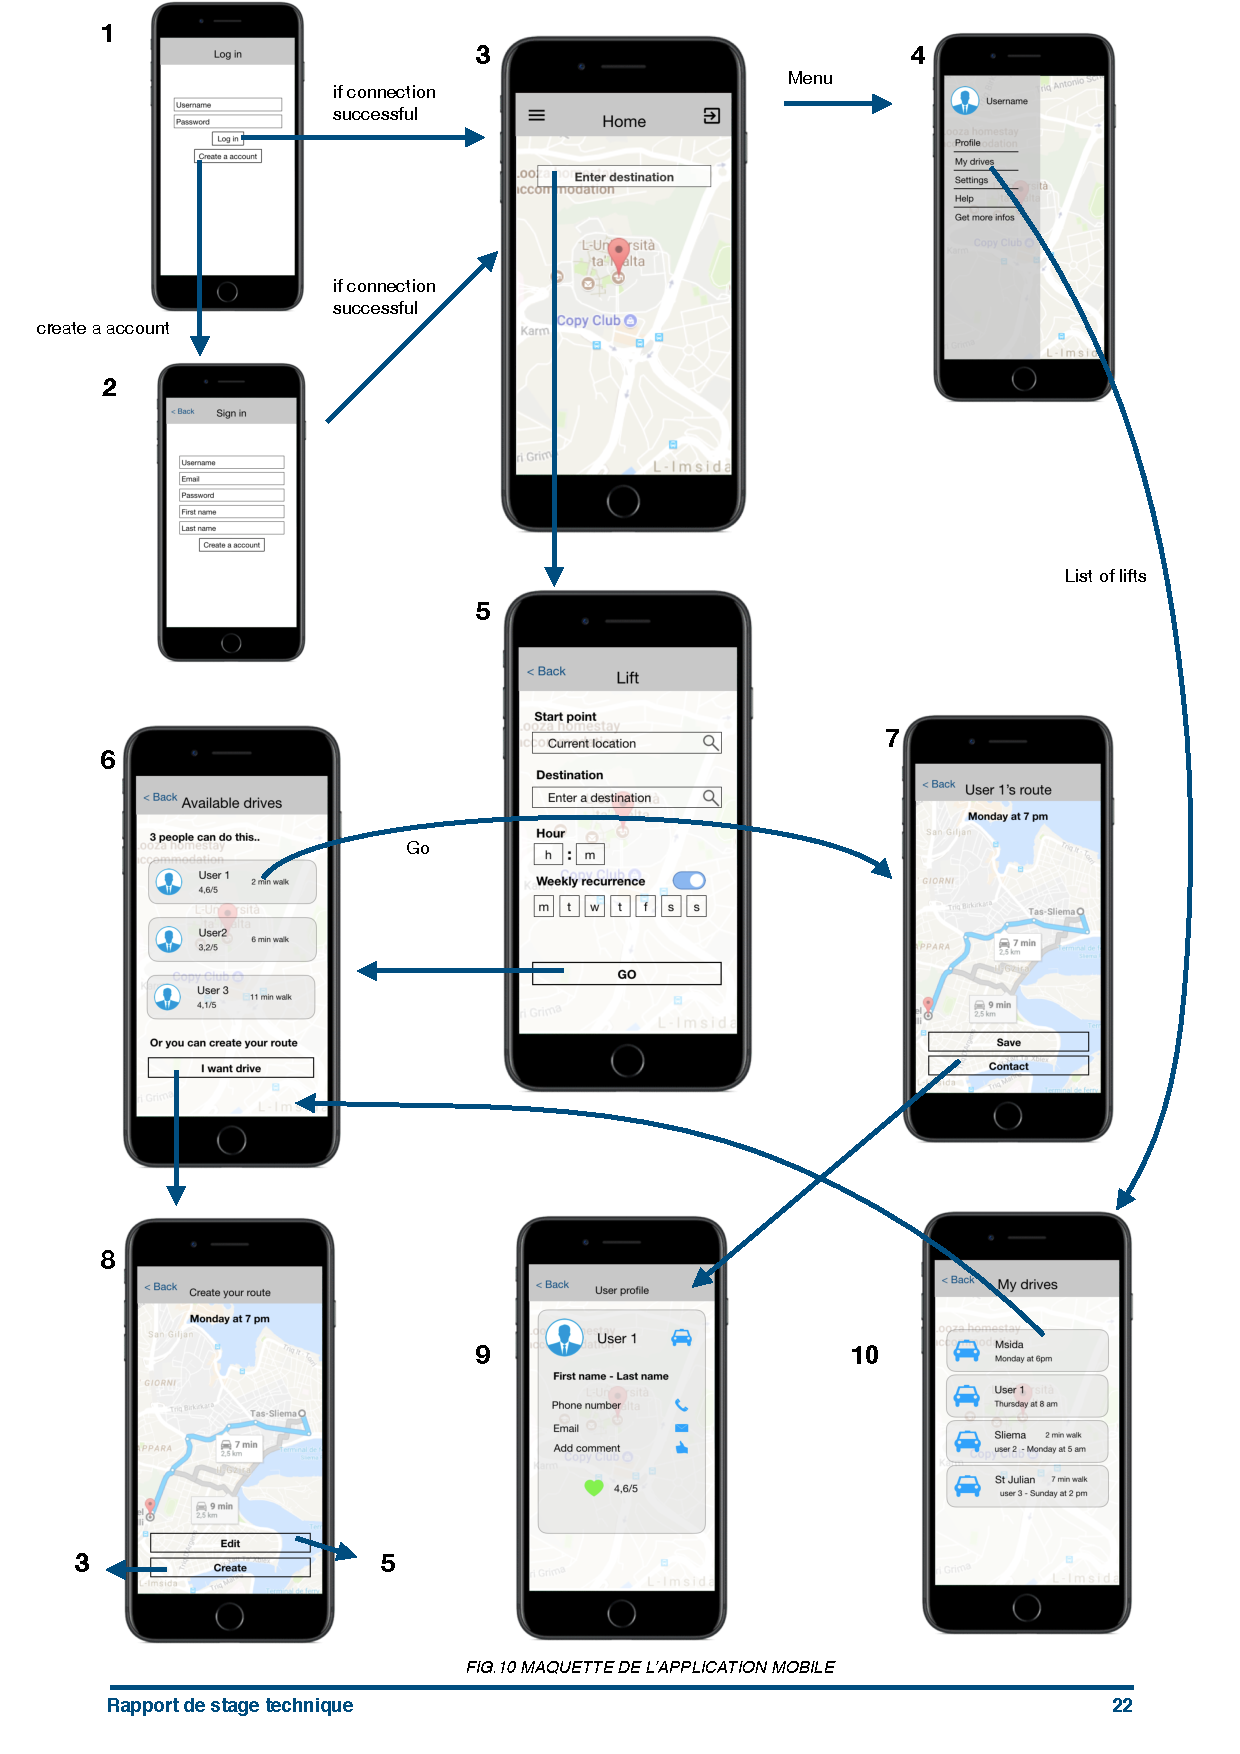
\includegraphics[page=1]{maquettes} 
\end{changemargin}